\section{Woche 15 - CSAF-Workshop beim BSI} \label{sec:bericht-wo-15-initial}

% 2023-12-11 bis 2023-12-15

\lweekdaymarginpar{\weekdayMondayShort, \weekdayTuesdayShort, \weekdayWednesdayShort}

Wie geplant begann ich die Woche mit der Recherche zum Thema CSA\@.
Die offizielle Dokumentation\footnote{\url{https://docs.oasis-open.org/csaf/csaf/v2.0/os/csaf-v2.0-os.html}} des Standards ist umfangreich, sodass ich den Großteil der Zeit damit verbrachte, die JSON-Strukturen und die Rollen der Teilnehmer zu verstehen.
CSAF definiert aber nicht nur das Format der Security Advisories, sondern auch deren Veröffentlichung, Bereitstellung, Aktualisierung und Verarbeitung durch Endnutzer.

Mir fiel auf, dass CSAF eine mir bisher noch nicht vorgekommene Methode zum Matchen von Produkten auf Advisories verwendet:
Zuerst muss pro Dokument ein Produktbaum verwendet werden, um durch die Knoten mit Bedingungen für die Nutzung der anliegenden Äste enthalten zu Blättern zu kommen, die jeweils ein Produkt identifizieren.
Diese Produkte werden dann in einer Sektion mit Kategorien wie \qt{affected} und \qt{not affected} aufgelistet, um herauszufinden, ob ein Produkt von einem Advisory betroffen ist.
Diese und weitere Erkenntnisse hielt ich in meinem Wiki-Eintrag fest und verließ Mittwoch das Büro etwas früher, um mich auf die Reise vorzubereiten.

\sweekdaymarginpar{\weekdayThursdayLong}

Donnerstag bin ich dann früh um 5:45 mit einem ICE nach München losgefahren, auf der glücklicherweise alles gut verlaufen ist und ich pünktlich in München angekommen bin.
Dort bin ich dann mit einer S-Bahn zum Flughafen gefahren, wo ich direkt zum Information Security Hub (ISH) gegangen bin, wo der Workshop stattfinden sollte.

Am Donnerstagmorgen fuhr ich um 5:45 Uhr mit dem ICE nach München, wo ich glücklicherweise pünktlich ankam.
Von dort ging es mit der S-Bahn zum Münchner Flughafen, wo der zum Information Security Hub (ISH) des BSI liegt, dem Ort des Workshops.

\begin{figure}[htbp] % here, top, bottom, separate page
    \centering
    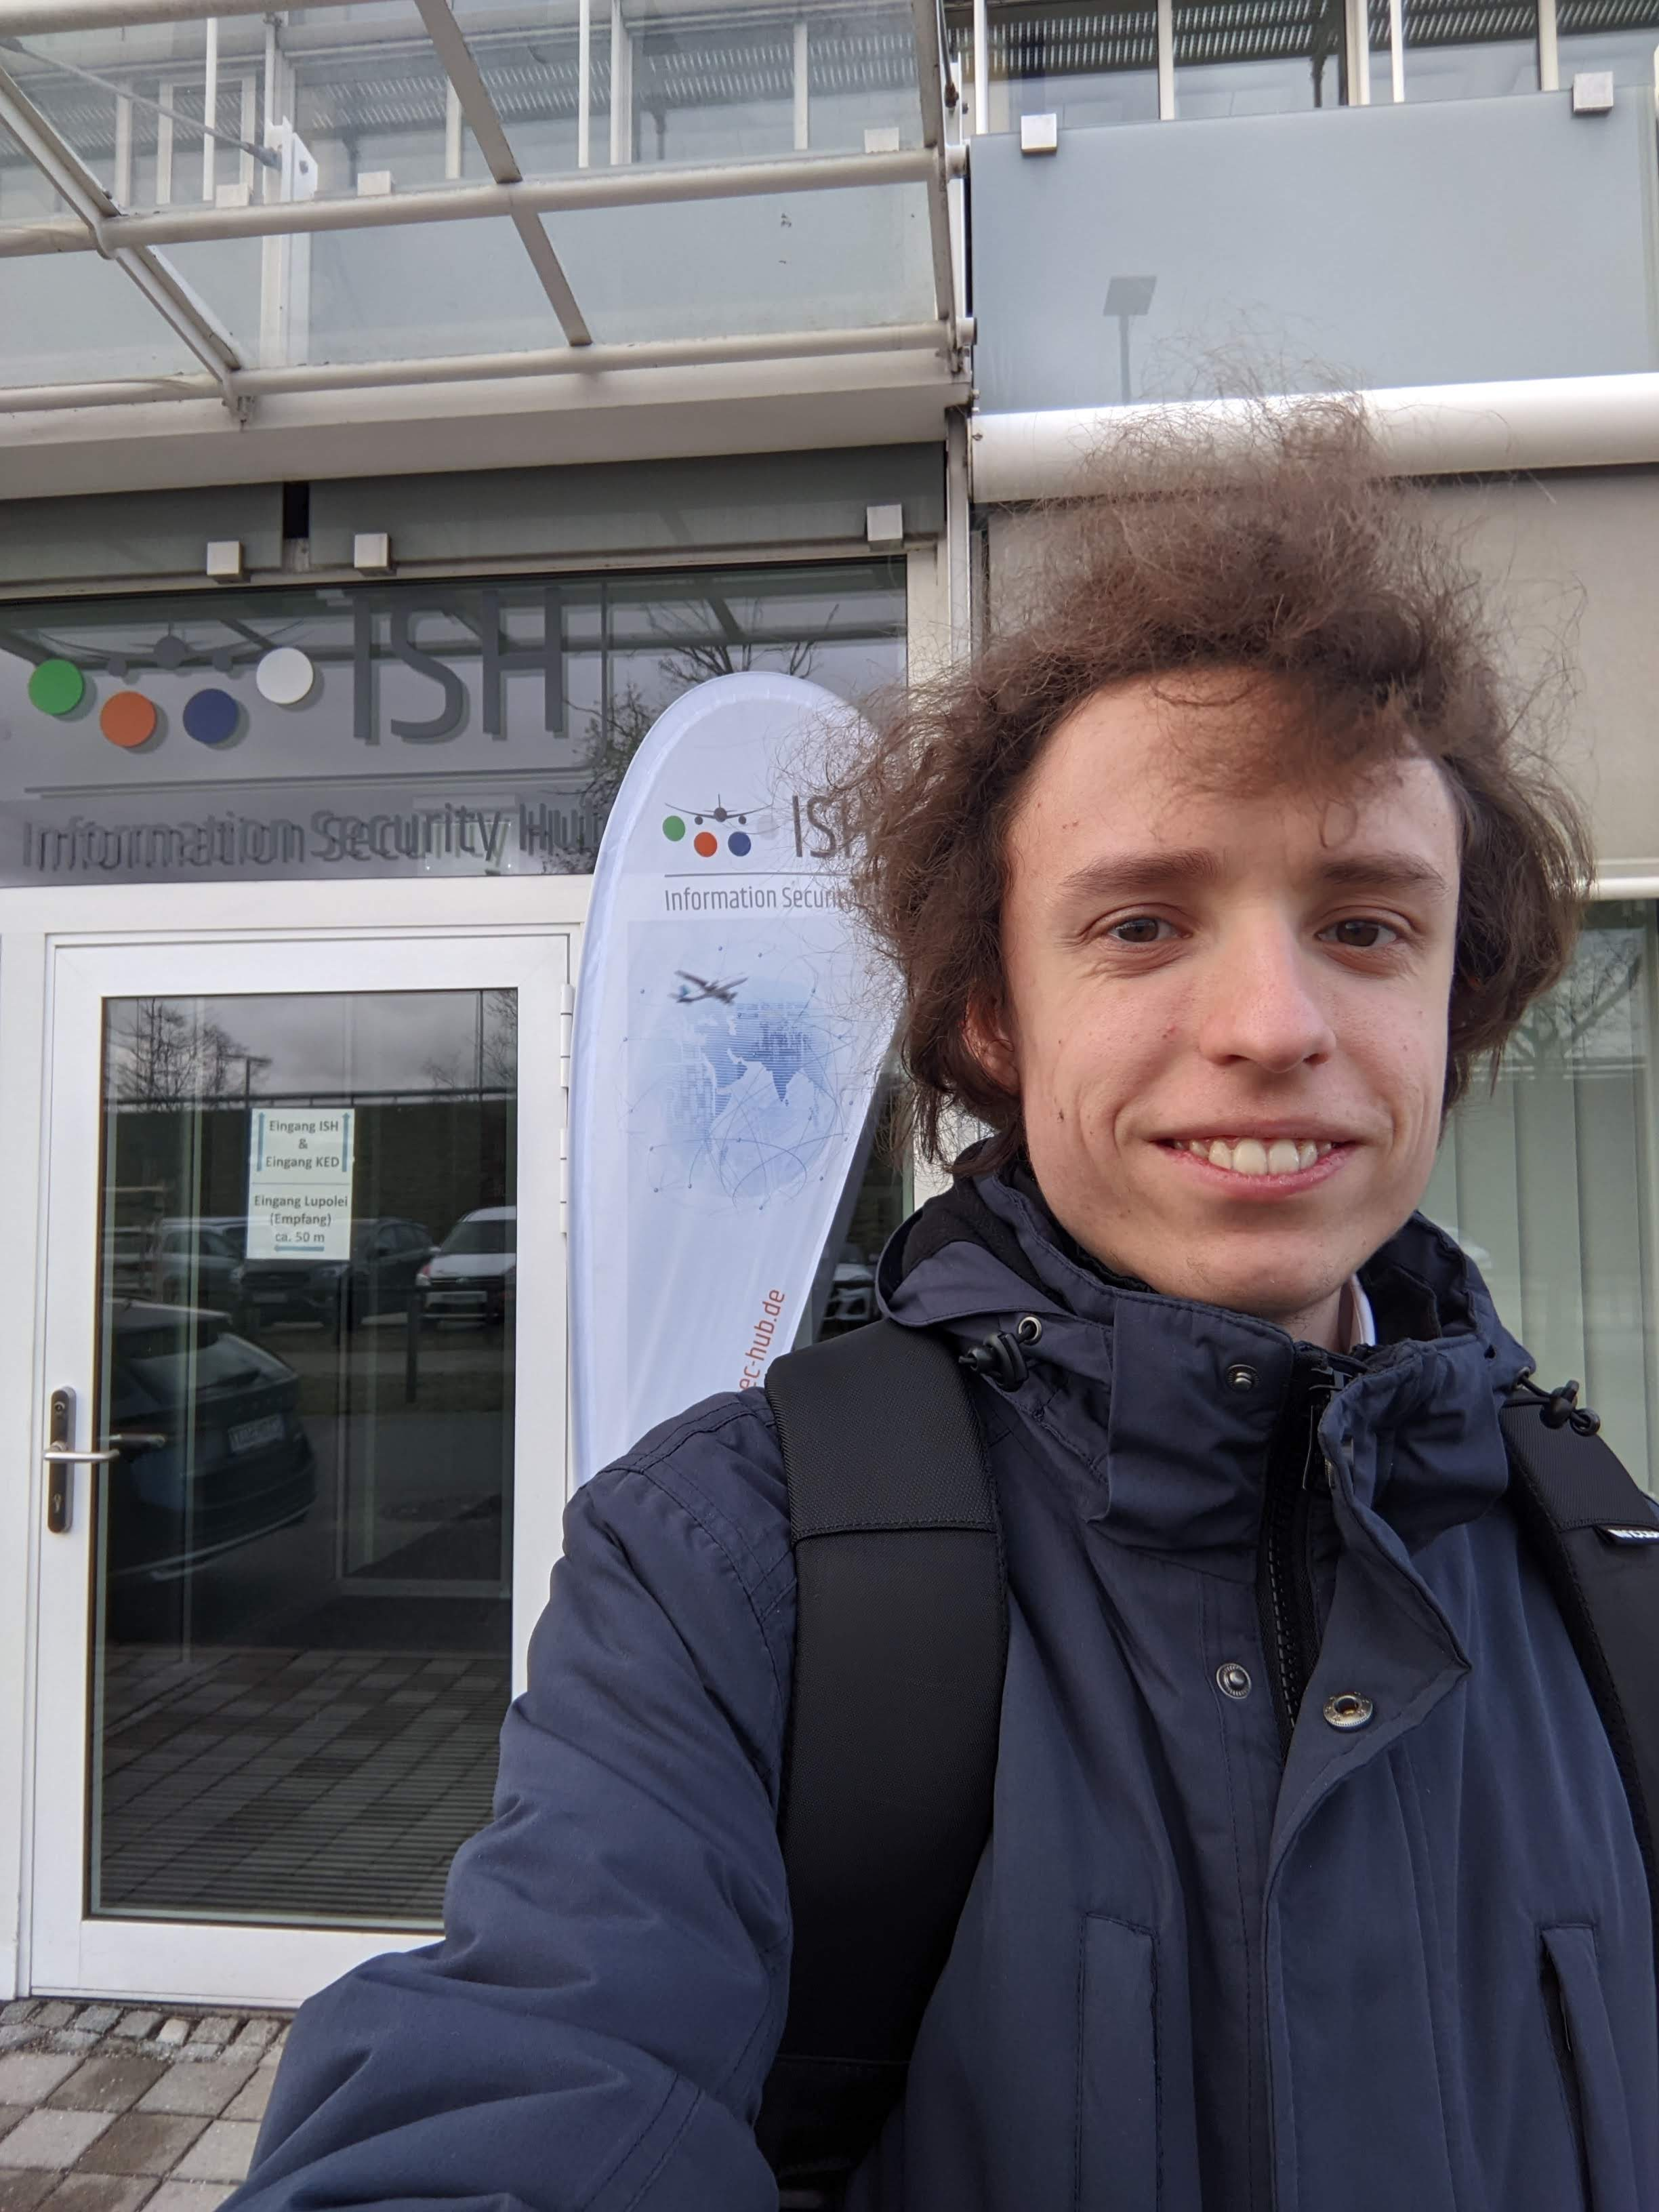
\includegraphics[width=0.5\textwidth, keepaspectratio]{res/img/2023-12-14-yan-vor-dem-ish-muenchen}
    \caption{Vor dem \qt{Information Security Hub} am Münchner Flughafen}
    \label{fig:yan-ish-csaf-muenchen-initial}
\end{figure}

Der vorherige Workshop war gerade zu Ende gegangen und die Teilnehmer, die auch am nächsten teilnehmen wollten, nutzten die 30-minütige Pause bis zum Beginn des nächsten, um sich auszutauschen.
Ich nutzte diese Gelegenheit, um einige Leute von Bosch und anderen Unternehmen kennenzulernen und mich mit ihnen über CSAF, über unser Unternehmen und andere Themen auszutauschen.

Der Workshop selbst bestand zur Hälfte aus einer theoretischen Präsentation, in der Begriffe, Rollen und Abläufe erklärt wurden, und zur anderen Hälfte aus praktischen Übungen an bereitgestellten Ubuntu-VMs.
Als Programmierer hatte ich keine Schwierigkeiten mit den Aufgaben und war oft der Einzige, der sie in der vorgegebenen Zeit abschließen konnte.
Das war vorteilhaft, denn so konnte ich noch mehr Menschen kennenlernen, indem ich auch ihnen bei den Aufgaben geholfen habe.

Besonders interessant waren allerdings die Diskussionen mit den Entwicklern des Standards.
Die Teilnehmenden hinterfragten einige Entscheidungen hinter CSAF und diskutierten, wie sich ihre individuellen Anwendungsfälle im Standard abbilden lassen.
Ich habe zu meinen eigenen Themen auch einige Fragen stellen können, wie unser Problem mit der uneindeutigen Produktidentifikation in verschiedenen Vendor- und Schwachstellendatenbanken und natürlich zum Thema CVSS, insbesondere zu den Herausforderungen mit vielen möglichen Vektoren für eine einzige Schwachstelle und zum neuen CVSS:4.0-Standard.

Nachdem der Workshop für den Tag beendet war und ich noch eine Weile am Buffet mit anderen Teilnehmern gesprochen hatte, ging ich zu meinem nahegelegenen Hotel.
Dort konnte ich den Tag nach einem kurzen Telefonat mit meinem Chef abschließen.

\sweekdaymarginpar{\weekdayFridayLong}

Freitagmorgen packte ich wieder früh um 5:30 im Hotel meine Sachen zusammen und checkte aus.
Zurück im ISH traf ich die Teilnehmer vom Vortag, konnte mich weiter austauschen und knüpfte weitere Kontakte.

Der Workshop begann mit einer weiteren Theorieeinheit zu den verschiedenen Rollen und Dokumentenarten, der Fokus lag aber heute auf der praktischen Anwendung des CSAF-Standards.
Unsere Aufgabe war es, die am Vortag eigens erstellten CSAF-Dokumente für die anderen Teilnehmer zugänglich zu machen, dann die der jeweils anderen herunterzuladen, zu validieren und zuletzt noch mit Python-Code zu verarbeiten.

Die Produktidentifikation war heute wieder ein großes Thema für die Teilnehmenden, da bisher vom Workshop nicht wirklich darauf eingegangen wurde, wie diese stattfinden sollte.
Für mich war das ebenfalls ein wichtiger Punkt, denn bei der \metaeffekt gibt es sogar eine Stelle, die sich nur mit der manuellen Zuordnung von Produkten aus Datenbanken zu unseren gescannten Komponenten befasst.
Eine richtige Lösung gibt es dafür scheinbar noch nicht, nur Ansätze, die so gut wie möglich in den Standard aufgenommen wurden.
Dies half zwar nicht wirklich unserem Problem weiter, es war aber auf jeden Fall gut zu hören, dass wir nicht die einzigen mit dieser Herausforderung sind.
In der dritten Version von CSAF möchten sie dieses Problem dann näher angehen.

Nach dem Ende des Workshops und abschließenden Gesprächen machte ich mich auf den Heimweg.
Dank einer Verspätung des ICE von Mannheim nach Heidelberg, wegen der die Zugbindung aufgehoben wurde, konnte ich eine frühere Verbindung nutzen und kam somit mehr als eine Stunde früher als geplant zu Hause an.
Die Erfahrungen teilte ich während der Fahrt mit meinem Chef, meine ausführlichen Notizen und Überlegungen würde ich dann in der folgenden Woche präsentieren.
